% ====== TAREA 2 MATEMATICAS APLICADAS ======
\documentclass{article}
\usepackage[utf8]{inputenc}
\usepackage[spanish]{babel}
\usepackage{amsmath, amsfonts, amssymb}
\usepackage{graphicx}
\usepackage[usenames]{color}
\usepackage[text={20cm,25cm},centering,top=1.5cm,bottom=1.5cm,letterpaper,showframe=false]{geometry}
\renewcommand{\baselinestretch}{1.5}
\parindent  = 0mm
\parskip    = 4mm
\definecolor{azul}{RGB}{10,80,190}
\definecolor{negro}{RGB}{0,0,0}
\definecolor{rojo}{RGB}{190,80,10}
\definecolor{verde}{RGB}{0,120,50}

\begin{document}
    \title{Tarea 2}
    \author{Careaga Carrillo Juan Manuel\\
            Quiróz Castañeda Edgar\\
            Soto Corderi Sandra del Mar}
    \date{Miércoles 10 de octubre de 2018}
    \maketitle
    \begin{enumerate}
        % Ejercicio 1
        \item {
            Encontrar la imagen de un triángulo con vérticies $(0,0)$, $(1,1)$
            y $(0,1)$ bajo la transformación $x=u^2$ y $y=v$.

            \color{azul}
            % Respuesta
        }

        % Ejercicio 2
        \item {
            Calcular
            \[
                \iint_{D}{e^{\frac{x-2y}{3x-y}}\,dA}
            \]
            con $D$ el paralelogramo acotado por las rectas $x-2y=0$, $x-2y=$,
            $3x-y=1$ y $3x-y=8$-

            \color{azul}
            % Respuesta
        }

        % Ejercicio 3
        \item {
            Hallar el volumen del elipsoide
            \[
                \frac{x^2}{a^2}+\frac{y^2}{b^2}+\frac{z^2}{c^2}\leq 1
            \]

            \color{azul}
            % Respuesta
        }

        % Ejercicio 4
        \item {
            Hallar el área acotada por la lemniscata
            \(
                \left(x^2+y^2\right)^2=2a^2\left(x^2-y^2\right)
            \).

            \color{azul}
            % Respuesta
        }

        % Ejercicio 5
        \item {
            Evaluar la integral iterada
            \[
                \int_{0}^{2}{
                    \int_{-\sqrt{2x-x^2}}^{\sqrt{2x-x^2}}{
                        \int_{0}^{x^2+y^2}{
                            \sqrt{x^2+y^2}
                        \,dz}
                    \,dy}
                \,dx}
            \]
            y bosquejar la región de integración $W$.

            \color{azul}
            % Respuesta
        }

        % Ejercicio 6
        \item {
            Calcular la masa del sólido que se encuentra fuera de la esfera
            $x^2+y^2+^z2=1$ y dentro de la esfera $x^2+y^2+z^2=2$ suponiendo
            que la densidad en un punto $P$ es directamente proporcional al
            cuadrado de la distancia de $P$ al centro de la esfera.

            \color{azul}
            % Respuesta
        }

        % Ejercicio 7
        \item {
            Determinar los números reales $\lambda$ para los que
            \[
                \iint_D {\frac{dA}{\left(x^2+y^2\right)^\lambda}}
            \]
            es convergente, con $D$ el disco unitario con centro en el origen.

            \color{azul}
            % Respuesta
            \begin{center}
                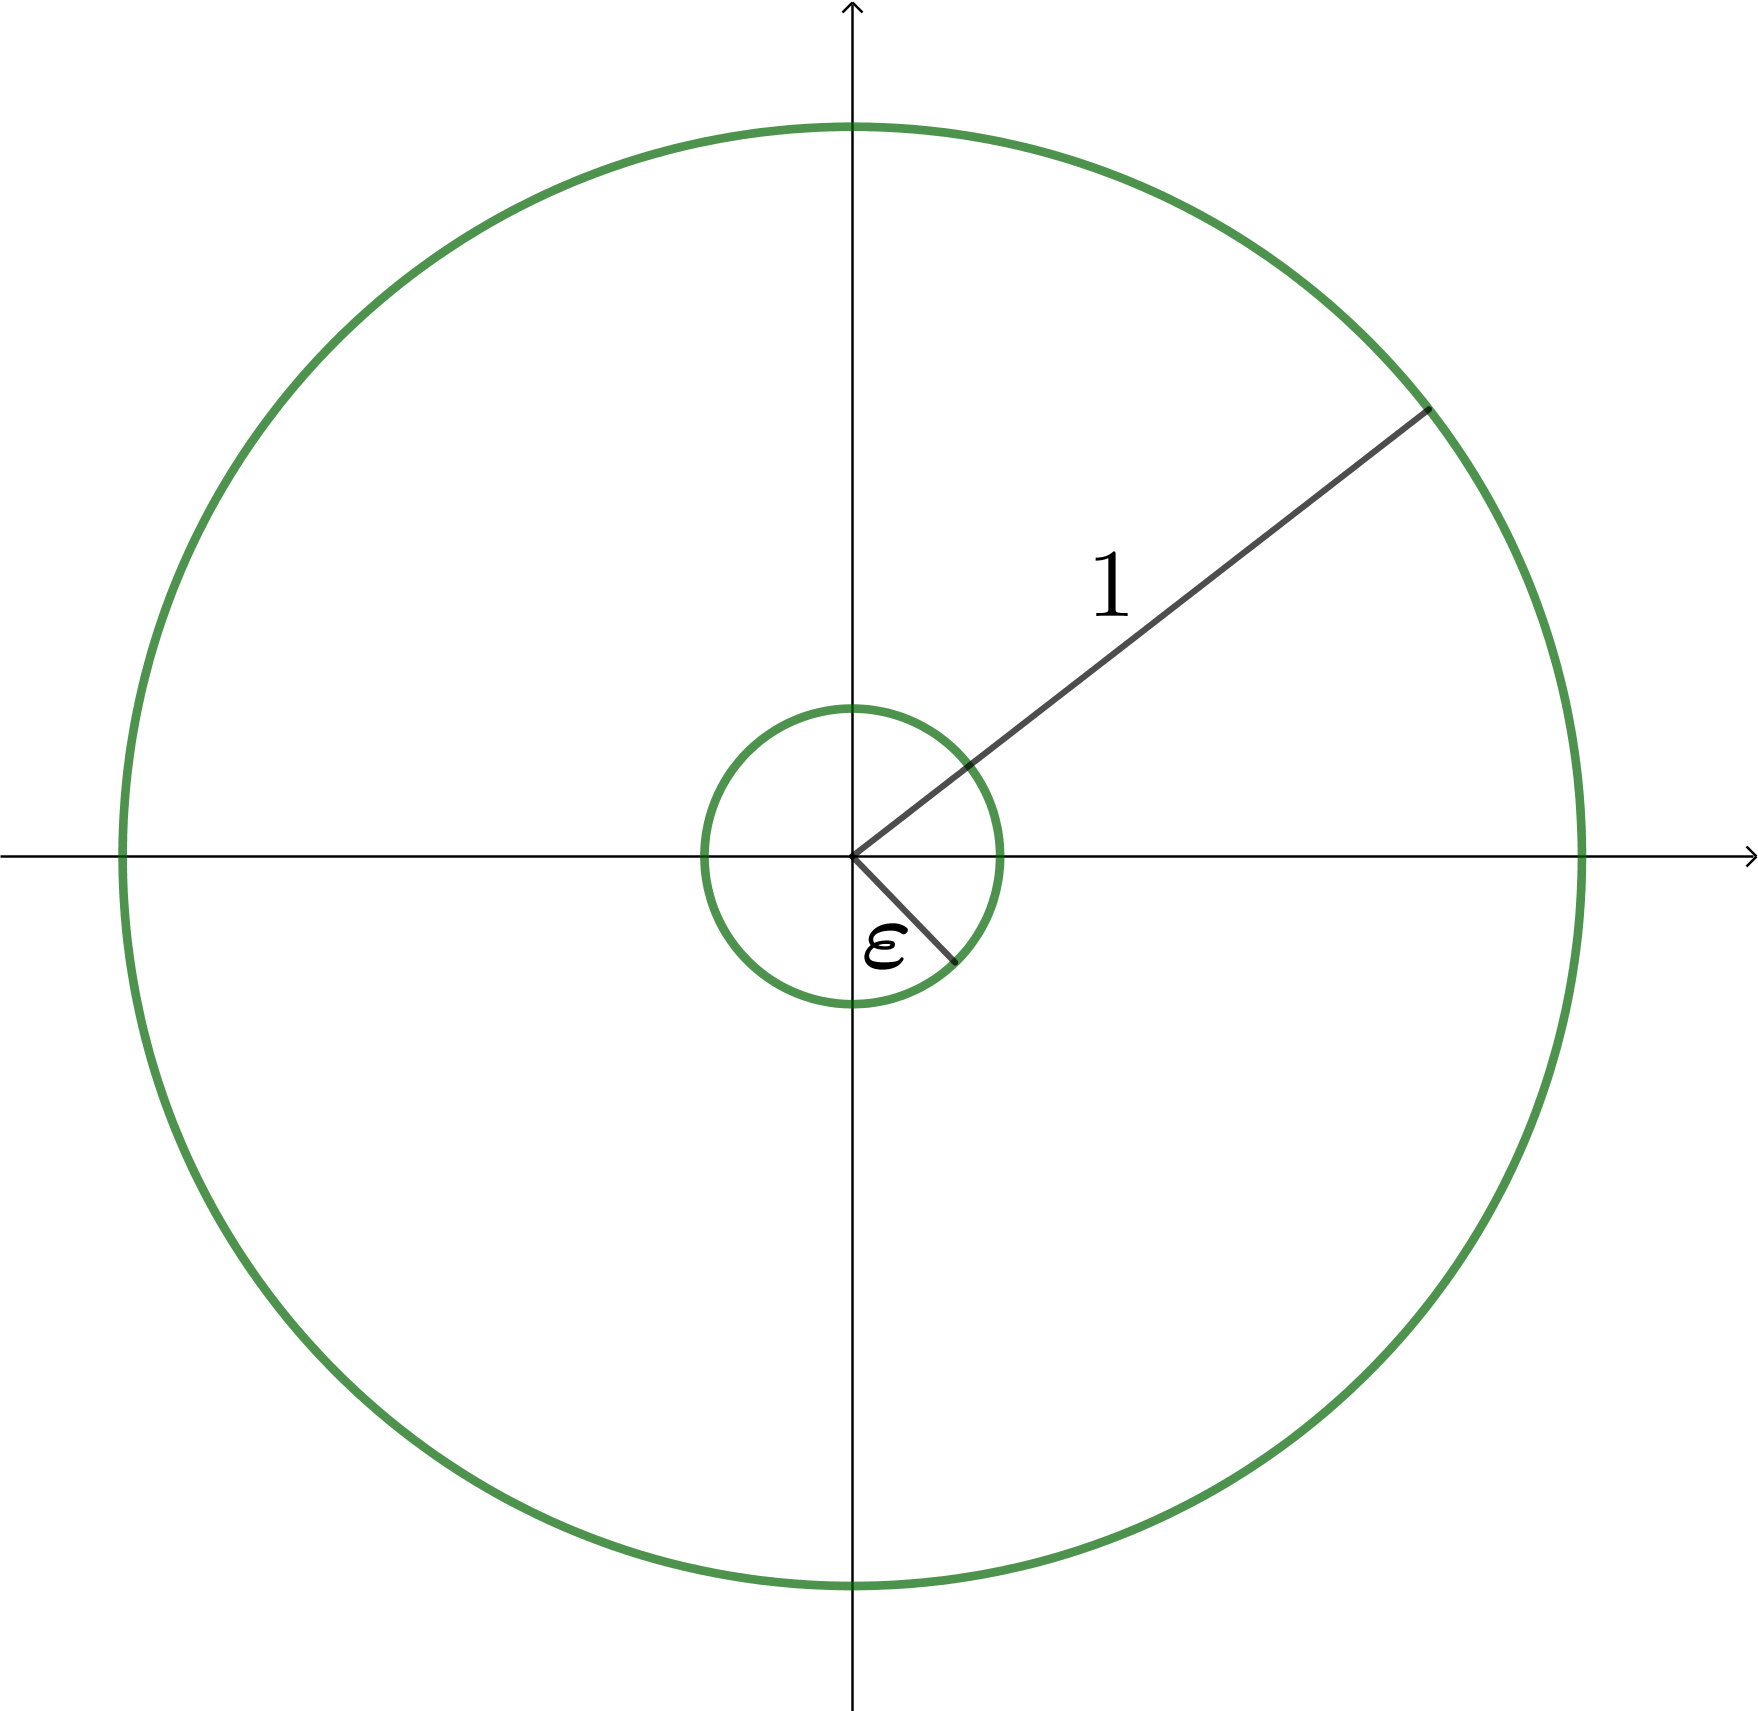
\includegraphics[width=4cm]{img/ej7.png}
            \end{center}
            La función $\displaystyle f(x)=\frac{1}{(x^2+y^2)^\lambda}$ no está
            definida cuando $x^2+y^2=0$, así que definimos una nueva región de
            integración $D_\varepsilon = \left\{(x,y)\in\mathbb{R}^2 |
            \varepsilon\leq x^2+y^2\leq 1\right\}$ y hacemos $\varepsilon
            \to 0$
            \[
                \iint_D {\frac{dA}{\left(x^2+y^2\right)^\lambda}}
                =\lim_{\varepsilon\to 0}{
                    \iint_{D_\varepsilon}{
                        \frac{dA}{\left(x^2+y^2\right)^\lambda}
                    }
                }
            \]
            para resolver la integral, conviene hacer una transformación a
            coordenadas polares
            \[
                \iint_D {\frac{dA}{\left(x^2+y^2\right)^\lambda}}
                =\int_{0}^{2\pi}{
                    \int_{0}^{1}{
                        \frac{r}{r^{2\lambda}}
                    \,dr}
                \,d\theta}
                =\lim_{\varepsilon\to 0}{
                    \int_{0}^{2\pi}{
                        \int_{\varepsilon}^{1}{
                            r^{1-2\lambda}
                        \,dr}
                    \,d\theta}
                }
            \]
            resolviendo la integral iterada (considerando $\lambda \ne 1$)
            \begin{align*}
                \lim_{\varepsilon\to 0}{
                    \int_{0}^{2\pi}{
                        \int_{\varepsilon}^{1}{
                            r^{1-2\lambda}
                        \,dr}
                    \,d\theta}
                }
                &=\lim_{\varepsilon\to 0}{
                    \int_{0}^{2\pi}{
                        \left[
                            \frac{r^{2-2\lambda}}
                                 {2-2\lambda}
                        \right]_{\varepsilon}^{1}
                    \,d\theta}
                }\\[.2cm]
                &=\lim_{\varepsilon\to 0}{
                    \int_{0}^{2\pi}{
                        \frac{1-\varepsilon^{2(1-\lambda)}}
                             {2(1-\lambda)}
                    \,d\theta}
                }\\[.2cm]
                &=\lim_{\varepsilon\to 0}{
                    \frac{2\pi[1-\varepsilon^{2(1-\lambda)}]}
                         {2(1-\lambda)}
                }\\[.2cm]
                &=\lim_{\varepsilon\to 0}{
                    \frac{\pi[1-\varepsilon^{2(1-\lambda)}]}
                         {1-\lambda}
                }
            \end{align*}
            Haciendo un análisis de ésta última expresión, concluimos que:
            \begin{itemize}
                \item si $\lambda>1$, entonces $1-\lambda>0$ y
                    $\varepsilon^{2(1-\lambda)}\to\infty$ (diverge)
                \item es cuando $\lambda<1$, entonces la integral converge.
            \end{itemize}
            
        }

        % Ejercicio 8
        \item {
            Calcular
            \[
                \iint_D {xye^{-\left(x^2+y^2\right)}\,dA}
            \]
            con $x\geq 0$ y $0\leq y\leq 1$.

            \color{azul}
            % Respuesta
            Notemos que la región de integración es infinita, como se ve en la
            siguiente figura
            \begin{center}
                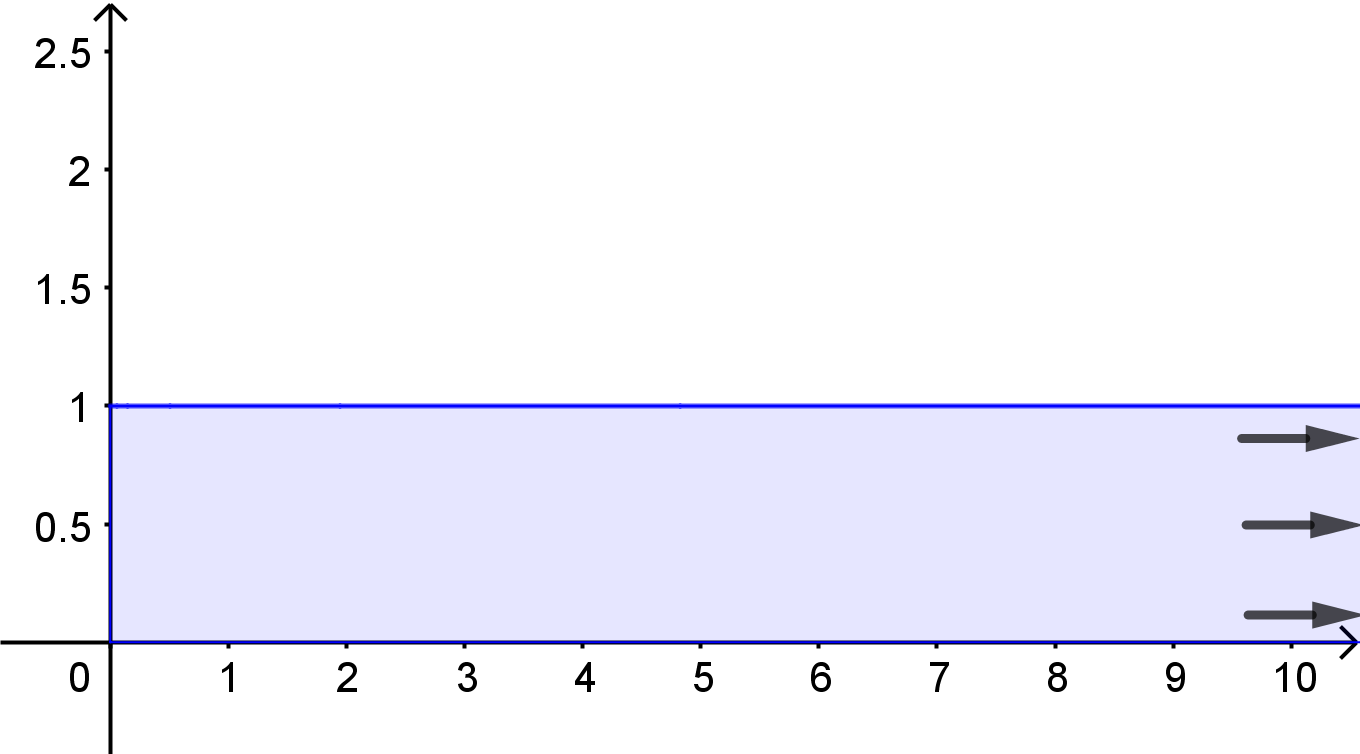
\includegraphics[width=5cm]{img/ej8.png}
            \end{center}
            Así que la integral iterada a resolver es
            \[
                \int_{0}^{\infty}{
                    \int_{0}^{1}{
                        xye^{-(x^2+y^2)}
                    \,dy}
                \,dx}
            \]
            Sustituimos ese infinito con una nueva variable $t$ y hacemos que
            ésta tienda hacia infinito
            \begin{align*}
                \lim_{t\to\infty}{
                    \int_{0}^{t}{
                        \int_{0}^{1}{
                            xye^{-(x^2+y^2)}
                        \,dy}
                    \,dx}
                }
                &=\lim_{t\to\infty}{
                    \int_{0}^{t}{
                        x\left[-\frac{1}{2}e^{-(x^2-y^2)}\right]_0^1
                    \,dx}
                }\\[.3cm]
                &=-\frac{1}{2}\lim_{t\to\infty}{
                    \int_{0}^{t}{
                        x\left[e^{-(x^2+1)}-e^{-x^2}\right]
                    \,dx}
                }\\[.3cm]
                &=-\frac{1}{2}\lim_{t\to\infty}{
                    \int_{0}^{t}{
                        xe^{-x^2}\left[e^{-1}-1\right]
                    \,dx}
                }\\[.3cm]
                &=-\frac{e^{-1}-1}{2}\lim_{t\to\infty}{
                    -\frac{1}{2}\left[-\frac{1}{2}e^{-x^2}\right]_{0}^{t}
                }\\[.3cm]
                &=\frac{e^{-1}-1}{4}\lim_{t\to\infty}{
                    \left(e^{-t^2}-1\right)
                }
            \end{align*}
            Simplificamos la expresión $\frac{e^{-1}-1}{4}=\frac{1-e}{4e}$ y al
            calcular el límite $e^{-t^2}\to 0$ por lo que el límite es
            $-1$ y el resultado de la integral es $\displaystyle\frac{e-1}{4e}$
        }
    \end{enumerate}
\end{document}
